\batchmode
\documentclass[twoside]{book}

% Packages required by doxygen
\usepackage{fixltx2e}
\usepackage{calc}
\usepackage{doxygen}
\usepackage[export]{adjustbox} % also loads graphicx
\usepackage{graphicx}
\usepackage[utf8]{inputenc}
\usepackage{makeidx}
\usepackage{multicol}
\usepackage{multirow}
\PassOptionsToPackage{warn}{textcomp}
\usepackage{textcomp}
\usepackage[nointegrals]{wasysym}
\usepackage[table]{xcolor}

% Font selection
\usepackage[T1]{fontenc}
\usepackage[scaled=.90]{helvet}
\usepackage{courier}
\usepackage{amssymb}
\usepackage{sectsty}
\renewcommand{\familydefault}{\sfdefault}
\allsectionsfont{%
  \fontseries{bc}\selectfont%
  \color{darkgray}%
}
\renewcommand{\DoxyLabelFont}{%
  \fontseries{bc}\selectfont%
  \color{darkgray}%
}
\newcommand{\+}{\discretionary{\mbox{\scriptsize$\hookleftarrow$}}{}{}}

% Page & text layout
\usepackage{geometry}
\geometry{%
  a4paper,%
  top=2.5cm,%
  bottom=2.5cm,%
  left=2.5cm,%
  right=2.5cm%
}
\tolerance=750
\hfuzz=15pt
\hbadness=750
\setlength{\emergencystretch}{15pt}
\setlength{\parindent}{0cm}
\setlength{\parskip}{3ex plus 2ex minus 2ex}
\makeatletter
\renewcommand{\paragraph}{%
  \@startsection{paragraph}{4}{0ex}{-1.0ex}{1.0ex}{%
    \normalfont\normalsize\bfseries\SS@parafont%
  }%
}
\renewcommand{\subparagraph}{%
  \@startsection{subparagraph}{5}{0ex}{-1.0ex}{1.0ex}{%
    \normalfont\normalsize\bfseries\SS@subparafont%
  }%
}
\makeatother

% Headers & footers
\usepackage{fancyhdr}
\pagestyle{fancyplain}
\fancyhead[LE]{\fancyplain{}{\bfseries\thepage}}
\fancyhead[CE]{\fancyplain{}{}}
\fancyhead[RE]{\fancyplain{}{\bfseries\leftmark}}
\fancyhead[LO]{\fancyplain{}{\bfseries\rightmark}}
\fancyhead[CO]{\fancyplain{}{}}
\fancyhead[RO]{\fancyplain{}{\bfseries\thepage}}
\fancyfoot[LE]{\fancyplain{}{}}
\fancyfoot[CE]{\fancyplain{}{}}
\fancyfoot[RE]{\fancyplain{}{\bfseries\scriptsize Generated by Doxygen }}
\fancyfoot[LO]{\fancyplain{}{\bfseries\scriptsize Generated by Doxygen }}
\fancyfoot[CO]{\fancyplain{}{}}
\fancyfoot[RO]{\fancyplain{}{}}
\renewcommand{\footrulewidth}{0.4pt}
\renewcommand{\chaptermark}[1]{%
  \markboth{#1}{}%
}
\renewcommand{\sectionmark}[1]{%
  \markright{\thesection\ #1}%
}

% Indices & bibliography
\usepackage{natbib}
\usepackage[titles]{tocloft}
\setcounter{tocdepth}{3}
\setcounter{secnumdepth}{5}
\makeindex

% Hyperlinks (required, but should be loaded last)
\usepackage{ifpdf}
\ifpdf
  \usepackage[pdftex,pagebackref=true]{hyperref}
\else
  \usepackage[ps2pdf,pagebackref=true]{hyperref}
\fi
\hypersetup{%
  colorlinks=true,%
  linkcolor=blue,%
  citecolor=blue,%
  unicode%
}

% Custom commands
\newcommand{\clearemptydoublepage}{%
  \newpage{\pagestyle{empty}\cleardoublepage}%
}

\usepackage{caption}
\captionsetup{labelsep=space,justification=centering,font={bf},singlelinecheck=off,skip=4pt,position=top}

%===== C O N T E N T S =====

\begin{document}

% Titlepage & ToC
\hypersetup{pageanchor=false,
             bookmarksnumbered=true,
             pdfencoding=unicode
            }
\pagenumbering{alph}
\pagenumbering{arabic}
\hypersetup{pageanchor=true}

%--- Begin generated contents ---
\chapter{Example problem\+: Adaptive solution of the 2D advection diffusion equation with flux boundary conditions}
\label{index}\hypertarget{index}{}\hypertarget{index_q}{}\section{A few quick questions...}\label{index_q}
Since {\ttfamily oomph-\/lib} is developed as open-\/source software, any evidence that the code is being downloaded and used is very helpful for us as it helps to justify our continued work on this project.

We would therefore be extremely grateful if you could provide the information requested in the form below. Pressing the \char`\"{}submit\char`\"{} button will get you to the actual download page.

{\bfseries Note\+:} 
\begin{DoxyItemize}
\item All information will be treated as confidential. 
\item If you provide your email address and check the appropriate box we will add you to our mailing list to inform you of upgrades and bug fixes to the code. Rest assured that the mailing list is {\bfseries very low volume} -- we have better things to do than to bombard you with email. 
\item If you still feel reluctant to provide any of the information requested, feel free to enter some dummy input. The form will check that {\bfseries some} information has been entered but entering your name as \char`\"{}\+Joe Cool\char`\"{} is perfectly acceptable -- this is to discourage people from not providing the information simply because they are too lazy to type... 
\end{DoxyItemize}



 







 

 \hypertarget{index_pdf}{}\section{P\+D\+F file}\label{index_pdf}
A \href{../latex/refman.pdf}{\tt pdf version} of this document is available. \end{document}

\chapter{Namespace Index}
\section{Namespace List}
Here is a list of all namespaces with brief descriptions\+:\begin{DoxyCompactList}
\item\contentsline{section}{\hyperlink{namespaceGlobal__Physical__Variables}{Global\+\_\+\+Physical\+\_\+\+Variables} \\*Global variables that represent physical properties }{\pageref{namespaceGlobal__Physical__Variables}}{}
\item\contentsline{section}{\hyperlink{namespaceoomph}{oomph} }{\pageref{namespaceoomph}}{}
\item\contentsline{section}{\hyperlink{namespacePhysical__Variables}{Physical\+\_\+\+Variables} \\*Namespace for the solution of 2D linear shell equation }{\pageref{namespacePhysical__Variables}}{}
\end{DoxyCompactList}

\chapter{Hierarchical Index}
\section{Class Hierarchy}
This inheritance list is sorted roughly, but not completely, alphabetically\+:\begin{DoxyCompactList}
\item Problem\begin{DoxyCompactList}
\item \contentsline{section}{Unstructured\+Solid\+Problem$<$ E\+L\+E\+M\+E\+NT $>$}{\pageref{classUnstructuredSolidProblem}}{}
\end{DoxyCompactList}
\end{DoxyCompactList}

\chapter{Class Index}
\section{Class List}
Here are the classes, structs, unions and interfaces with brief descriptions\+:\begin{DoxyCompactList}
\item\contentsline{section}{\hyperlink{classPMLProblem}{P\+M\+L\+Problem$<$ E\+L\+E\+M\+E\+N\+T $>$} }{\pageref{classPMLProblem}}{}
\item\contentsline{section}{\hyperlink{classGlobalParameters_1_1TestPMLMapping}{Global\+Parameters\+::\+Test\+P\+M\+L\+Mapping} }{\pageref{classGlobalParameters_1_1TestPMLMapping}}{}
\end{DoxyCompactList}

\chapter{File Index}
\section{File List}
Here is a list of all files with brief descriptions\+:\begin{DoxyCompactList}
\item\contentsline{section}{\hyperlink{jeffery__orbit_8cc}{jeffery\+\_\+orbit.\+cc} }{\pageref{jeffery__orbit_8cc}}{}
\item\contentsline{section}{\hyperlink{jeffery__orbit_8txt__doxygenified_8h}{jeffery\+\_\+orbit.\+txt\+\_\+doxygenified.\+h} }{\pageref{jeffery__orbit_8txt__doxygenified_8h}}{}
\item\contentsline{section}{\hyperlink{my__taylor__hood__elements_8h}{my\+\_\+taylor\+\_\+hood\+\_\+elements.\+h} }{\pageref{my__taylor__hood__elements_8h}}{}
\end{DoxyCompactList}

\chapter{Namespace Documentation}
\hypertarget{namespaceTanhSolnForAdvectionDiffusion}{}\section{Tanh\+Soln\+For\+Advection\+Diffusion Namespace Reference}
\label{namespaceTanhSolnForAdvectionDiffusion}\index{Tanh\+Soln\+For\+Advection\+Diffusion@{Tanh\+Soln\+For\+Advection\+Diffusion}}
\subsection*{Functions}
\begin{DoxyCompactItemize}
\item 
void \hyperlink{namespaceTanhSolnForAdvectionDiffusion_ae4c9ed0a4f123ec8e634f0cc45bfcebc}{get\+\_\+exact\+\_\+u} (const Vector$<$ double $>$ \&x, Vector$<$ double $>$ \&u)
\begin{DoxyCompactList}\small\item\em Exact solution as a Vector. \end{DoxyCompactList}\item 
void \hyperlink{namespaceTanhSolnForAdvectionDiffusion_af302dc41c1e494b3430fe6654bd1fd39}{get\+\_\+exact\+\_\+u} (const Vector$<$ double $>$ \&x, double \&u)
\begin{DoxyCompactList}\small\item\em Exact solution as a scalar. \end{DoxyCompactList}\item 
void \hyperlink{namespaceTanhSolnForAdvectionDiffusion_aaa1aa95713b02b211812fdd18eeaa369}{source\+\_\+function} (const Vector$<$ double $>$ \&x\+\_\+vect, double \&source)
\begin{DoxyCompactList}\small\item\em Source function required to make the solution above an exact solution. \end{DoxyCompactList}\item 
void \hyperlink{namespaceTanhSolnForAdvectionDiffusion_ab40e93031d34986762c69616c3c8b065}{wind\+\_\+function} (const Vector$<$ double $>$ \&x, Vector$<$ double $>$ \&wind)
\begin{DoxyCompactList}\small\item\em Wind. \end{DoxyCompactList}\item 
void \hyperlink{namespaceTanhSolnForAdvectionDiffusion_a4016f2f5bd0c82061bee09043dc8e8e6}{tanh\+\_\+profile} (const Vector$<$ double $>$ \&x, Vector$<$ double $>$ \&u)
\begin{DoxyCompactList}\small\item\em Tanh profile for assignment of boundary conditons as a Vector. \end{DoxyCompactList}\item 
void \hyperlink{namespaceTanhSolnForAdvectionDiffusion_afee88c1e0f93cc56d06c2e94aaf8449c}{tanh\+\_\+profile} (const Vector$<$ double $>$ \&x, double \&u)
\begin{DoxyCompactList}\small\item\em Tanh profile for assignment of boundary conditons as a Vector. \end{DoxyCompactList}\end{DoxyCompactItemize}
\subsection*{Variables}
\begin{DoxyCompactItemize}
\item 
double \hyperlink{namespaceTanhSolnForAdvectionDiffusion_aeba486af70e92ab7eec1da3ce44d51ee}{Peclet} =200.\+0
\begin{DoxyCompactList}\small\item\em Peclet number. \end{DoxyCompactList}\item 
double \hyperlink{namespaceTanhSolnForAdvectionDiffusion_a4d202e8ac48cc75f760ef40681402ec7}{Alpha}
\begin{DoxyCompactList}\small\item\em Parameter for steepness of step. \end{DoxyCompactList}\item 
double \hyperlink{namespaceTanhSolnForAdvectionDiffusion_a236bf82c661189623706b7c9d9b0c52f}{Tan\+Phi}
\begin{DoxyCompactList}\small\item\em Parameter for angle of step. \end{DoxyCompactList}\end{DoxyCompactItemize}


\subsection{Detailed Description}
Namespace for exact solution for Advection\+Diffusion equation with \char`\"{}sharp\char`\"{} step

Namespace for physical parameters and boundary conditions \char`\"{}sharp\char`\"{} step 

\subsection{Function Documentation}
\mbox{\Hypertarget{namespaceTanhSolnForAdvectionDiffusion_ae4c9ed0a4f123ec8e634f0cc45bfcebc}\label{namespaceTanhSolnForAdvectionDiffusion_ae4c9ed0a4f123ec8e634f0cc45bfcebc}} 
\index{Tanh\+Soln\+For\+Advection\+Diffusion@{Tanh\+Soln\+For\+Advection\+Diffusion}!get\+\_\+exact\+\_\+u@{get\+\_\+exact\+\_\+u}}
\index{get\+\_\+exact\+\_\+u@{get\+\_\+exact\+\_\+u}!Tanh\+Soln\+For\+Advection\+Diffusion@{Tanh\+Soln\+For\+Advection\+Diffusion}}
\subsubsection{\texorpdfstring{get\+\_\+exact\+\_\+u()}{get\_exact\_u()}\hspace{0.1cm}{\footnotesize\ttfamily [1/2]}}
{\footnotesize\ttfamily void Tanh\+Soln\+For\+Advection\+Diffusion\+::get\+\_\+exact\+\_\+u (\begin{DoxyParamCaption}\item[{const Vector$<$ double $>$ \&}]{x,  }\item[{Vector$<$ double $>$ \&}]{u }\end{DoxyParamCaption})}



Exact solution as a Vector. 



Definition at line 63 of file two\+\_\+d\+\_\+adv\+\_\+diff\+\_\+adapt.\+cc.



Referenced by Refineable\+Advection\+Diffusion\+Problem$<$ E\+L\+E\+M\+E\+N\+T $>$\+::actions\+\_\+before\+\_\+newton\+\_\+solve(), and Refineable\+Advection\+Diffusion\+Problem$<$ E\+L\+E\+M\+E\+N\+T $>$\+::doc\+\_\+solution().

\mbox{\Hypertarget{namespaceTanhSolnForAdvectionDiffusion_af302dc41c1e494b3430fe6654bd1fd39}\label{namespaceTanhSolnForAdvectionDiffusion_af302dc41c1e494b3430fe6654bd1fd39}} 
\index{Tanh\+Soln\+For\+Advection\+Diffusion@{Tanh\+Soln\+For\+Advection\+Diffusion}!get\+\_\+exact\+\_\+u@{get\+\_\+exact\+\_\+u}}
\index{get\+\_\+exact\+\_\+u@{get\+\_\+exact\+\_\+u}!Tanh\+Soln\+For\+Advection\+Diffusion@{Tanh\+Soln\+For\+Advection\+Diffusion}}
\subsubsection{\texorpdfstring{get\+\_\+exact\+\_\+u()}{get\_exact\_u()}\hspace{0.1cm}{\footnotesize\ttfamily [2/2]}}
{\footnotesize\ttfamily void Tanh\+Soln\+For\+Advection\+Diffusion\+::get\+\_\+exact\+\_\+u (\begin{DoxyParamCaption}\item[{const Vector$<$ double $>$ \&}]{x,  }\item[{double \&}]{u }\end{DoxyParamCaption})}



Exact solution as a scalar. 



Definition at line 69 of file two\+\_\+d\+\_\+adv\+\_\+diff\+\_\+adapt.\+cc.

\mbox{\Hypertarget{namespaceTanhSolnForAdvectionDiffusion_aaa1aa95713b02b211812fdd18eeaa369}\label{namespaceTanhSolnForAdvectionDiffusion_aaa1aa95713b02b211812fdd18eeaa369}} 
\index{Tanh\+Soln\+For\+Advection\+Diffusion@{Tanh\+Soln\+For\+Advection\+Diffusion}!source\+\_\+function@{source\+\_\+function}}
\index{source\+\_\+function@{source\+\_\+function}!Tanh\+Soln\+For\+Advection\+Diffusion@{Tanh\+Soln\+For\+Advection\+Diffusion}}
\subsubsection{\texorpdfstring{source\+\_\+function()}{source\_function()}}
{\footnotesize\ttfamily void Tanh\+Soln\+For\+Advection\+Diffusion\+::source\+\_\+function (\begin{DoxyParamCaption}\item[{const Vector$<$ double $>$ \&}]{x\+\_\+vect,  }\item[{double \&}]{source }\end{DoxyParamCaption})}



Source function required to make the solution above an exact solution. 

Zero source function. 

Definition at line 75 of file two\+\_\+d\+\_\+adv\+\_\+diff\+\_\+adapt.\+cc.



Referenced by main(), and tanh\+\_\+profile().

\mbox{\Hypertarget{namespaceTanhSolnForAdvectionDiffusion_a4016f2f5bd0c82061bee09043dc8e8e6}\label{namespaceTanhSolnForAdvectionDiffusion_a4016f2f5bd0c82061bee09043dc8e8e6}} 
\index{Tanh\+Soln\+For\+Advection\+Diffusion@{Tanh\+Soln\+For\+Advection\+Diffusion}!tanh\+\_\+profile@{tanh\+\_\+profile}}
\index{tanh\+\_\+profile@{tanh\+\_\+profile}!Tanh\+Soln\+For\+Advection\+Diffusion@{Tanh\+Soln\+For\+Advection\+Diffusion}}
\subsubsection{\texorpdfstring{tanh\+\_\+profile()}{tanh\_profile()}\hspace{0.1cm}{\footnotesize\ttfamily [1/2]}}
{\footnotesize\ttfamily void Tanh\+Soln\+For\+Advection\+Diffusion\+::tanh\+\_\+profile (\begin{DoxyParamCaption}\item[{const Vector$<$ double $>$ \&}]{x,  }\item[{Vector$<$ double $>$ \&}]{u }\end{DoxyParamCaption})}



Tanh profile for assignment of boundary conditons as a Vector. 



Definition at line 62 of file two\+\_\+d\+\_\+adv\+\_\+diff\+\_\+adapt2.\+cc.



Referenced by Refineable\+Advection\+Diffusion\+Problem$<$ E\+L\+E\+M\+E\+N\+T $>$\+::mesh\+\_\+pt().

\mbox{\Hypertarget{namespaceTanhSolnForAdvectionDiffusion_afee88c1e0f93cc56d06c2e94aaf8449c}\label{namespaceTanhSolnForAdvectionDiffusion_afee88c1e0f93cc56d06c2e94aaf8449c}} 
\index{Tanh\+Soln\+For\+Advection\+Diffusion@{Tanh\+Soln\+For\+Advection\+Diffusion}!tanh\+\_\+profile@{tanh\+\_\+profile}}
\index{tanh\+\_\+profile@{tanh\+\_\+profile}!Tanh\+Soln\+For\+Advection\+Diffusion@{Tanh\+Soln\+For\+Advection\+Diffusion}}
\subsubsection{\texorpdfstring{tanh\+\_\+profile()}{tanh\_profile()}\hspace{0.1cm}{\footnotesize\ttfamily [2/2]}}
{\footnotesize\ttfamily void Tanh\+Soln\+For\+Advection\+Diffusion\+::tanh\+\_\+profile (\begin{DoxyParamCaption}\item[{const Vector$<$ double $>$ \&}]{x,  }\item[{double \&}]{u }\end{DoxyParamCaption})}



Tanh profile for assignment of boundary conditons as a Vector. 



Definition at line 68 of file two\+\_\+d\+\_\+adv\+\_\+diff\+\_\+adapt2.\+cc.



References source\+\_\+function(), and wind\+\_\+function().

\mbox{\Hypertarget{namespaceTanhSolnForAdvectionDiffusion_ab40e93031d34986762c69616c3c8b065}\label{namespaceTanhSolnForAdvectionDiffusion_ab40e93031d34986762c69616c3c8b065}} 
\index{Tanh\+Soln\+For\+Advection\+Diffusion@{Tanh\+Soln\+For\+Advection\+Diffusion}!wind\+\_\+function@{wind\+\_\+function}}
\index{wind\+\_\+function@{wind\+\_\+function}!Tanh\+Soln\+For\+Advection\+Diffusion@{Tanh\+Soln\+For\+Advection\+Diffusion}}
\subsubsection{\texorpdfstring{wind\+\_\+function()}{wind\_function()}}
{\footnotesize\ttfamily void Tanh\+Soln\+For\+Advection\+Diffusion\+::wind\+\_\+function (\begin{DoxyParamCaption}\item[{const Vector$<$ double $>$ \&}]{x,  }\item[{Vector$<$ double $>$ \&}]{wind }\end{DoxyParamCaption})}



Wind. 

Wind\+: Recirculating cells. 

Definition at line 88 of file two\+\_\+d\+\_\+adv\+\_\+diff\+\_\+adapt.\+cc.



Referenced by main(), and tanh\+\_\+profile().



\subsection{Variable Documentation}
\mbox{\Hypertarget{namespaceTanhSolnForAdvectionDiffusion_a4d202e8ac48cc75f760ef40681402ec7}\label{namespaceTanhSolnForAdvectionDiffusion_a4d202e8ac48cc75f760ef40681402ec7}} 
\index{Tanh\+Soln\+For\+Advection\+Diffusion@{Tanh\+Soln\+For\+Advection\+Diffusion}!Alpha@{Alpha}}
\index{Alpha@{Alpha}!Tanh\+Soln\+For\+Advection\+Diffusion@{Tanh\+Soln\+For\+Advection\+Diffusion}}
\subsubsection{\texorpdfstring{Alpha}{Alpha}}
{\footnotesize\ttfamily double Tanh\+Soln\+For\+Advection\+Diffusion\+::\+Alpha}



Parameter for steepness of step. 

Parameter for steepness of step in tanh profile. 

Definition at line 57 of file two\+\_\+d\+\_\+adv\+\_\+diff\+\_\+adapt.\+cc.



Referenced by main().

\mbox{\Hypertarget{namespaceTanhSolnForAdvectionDiffusion_aeba486af70e92ab7eec1da3ce44d51ee}\label{namespaceTanhSolnForAdvectionDiffusion_aeba486af70e92ab7eec1da3ce44d51ee}} 
\index{Tanh\+Soln\+For\+Advection\+Diffusion@{Tanh\+Soln\+For\+Advection\+Diffusion}!Peclet@{Peclet}}
\index{Peclet@{Peclet}!Tanh\+Soln\+For\+Advection\+Diffusion@{Tanh\+Soln\+For\+Advection\+Diffusion}}
\subsubsection{\texorpdfstring{Peclet}{Peclet}}
{\footnotesize\ttfamily double Tanh\+Soln\+For\+Advection\+Diffusion\+::\+Peclet =200.\+0}



Peclet number. 



Definition at line 54 of file two\+\_\+d\+\_\+adv\+\_\+diff\+\_\+adapt.\+cc.



Referenced by Refineable\+Advection\+Diffusion\+Problem$<$ E\+L\+E\+M\+E\+N\+T $>$\+::mesh\+\_\+pt(), and Refineable\+Advection\+Diffusion\+Problem$<$ E\+L\+E\+M\+E\+N\+T $>$\+::\+Refineable\+Advection\+Diffusion\+Problem().

\mbox{\Hypertarget{namespaceTanhSolnForAdvectionDiffusion_a236bf82c661189623706b7c9d9b0c52f}\label{namespaceTanhSolnForAdvectionDiffusion_a236bf82c661189623706b7c9d9b0c52f}} 
\index{Tanh\+Soln\+For\+Advection\+Diffusion@{Tanh\+Soln\+For\+Advection\+Diffusion}!Tan\+Phi@{Tan\+Phi}}
\index{Tan\+Phi@{Tan\+Phi}!Tanh\+Soln\+For\+Advection\+Diffusion@{Tanh\+Soln\+For\+Advection\+Diffusion}}
\subsubsection{\texorpdfstring{Tan\+Phi}{TanPhi}}
{\footnotesize\ttfamily double Tanh\+Soln\+For\+Advection\+Diffusion\+::\+Tan\+Phi}



Parameter for angle of step. 

Parameter for angle of step in tanh profile. 

Definition at line 60 of file two\+\_\+d\+\_\+adv\+\_\+diff\+\_\+adapt.\+cc.



Referenced by main().


\chapter{Class Documentation}
\hypertarget{classTwoMeshFluxAdvectionDiffusionProblem}{}\section{Two\+Mesh\+Flux\+Advection\+Diffusion\+Problem$<$ E\+L\+E\+M\+E\+NT $>$ Class Template Reference}
\label{classTwoMeshFluxAdvectionDiffusionProblem}\index{Two\+Mesh\+Flux\+Advection\+Diffusion\+Problem$<$ E\+L\+E\+M\+E\+N\+T $>$@{Two\+Mesh\+Flux\+Advection\+Diffusion\+Problem$<$ E\+L\+E\+M\+E\+N\+T $>$}}
Inheritance diagram for Two\+Mesh\+Flux\+Advection\+Diffusion\+Problem$<$ E\+L\+E\+M\+E\+NT $>$\+:\begin{figure}[H]
\begin{center}
\leavevmode
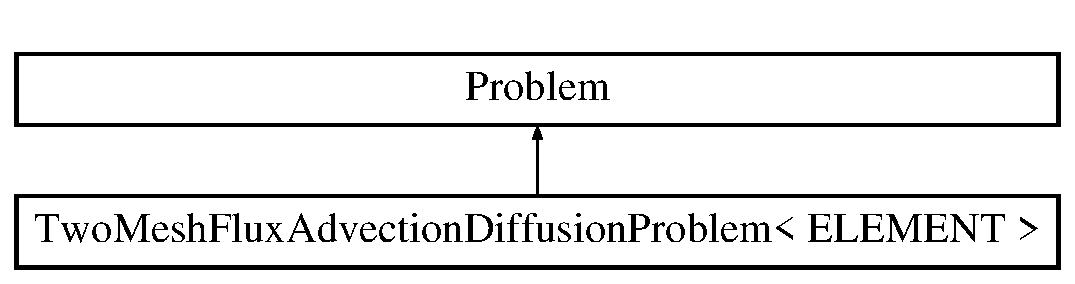
\includegraphics[height=2.000000cm]{classTwoMeshFluxAdvectionDiffusionProblem}
\end{center}
\end{figure}
\subsection*{Public Member Functions}
\begin{DoxyCompactItemize}
\item 
\hyperlink{classTwoMeshFluxAdvectionDiffusionProblem_a7f3ec24317465521cb84212d1c2dc662}{Two\+Mesh\+Flux\+Advection\+Diffusion\+Problem} (Advection\+Diffusion\+Equations$<$ 2 $>$\+::Advection\+Diffusion\+Source\+Fct\+Pt source\+\_\+fct\+\_\+pt, Advection\+Diffusion\+Equations$<$ 2 $>$\+::Advection\+Diffusion\+Wind\+Fct\+Pt wind\+\_\+fct\+\_\+pt)
\begin{DoxyCompactList}\small\item\em Constructor\+: Pass pointer to source and wind functions. \end{DoxyCompactList}\item 
\hyperlink{classTwoMeshFluxAdvectionDiffusionProblem_a65445b9eb9c01680d8137d1fdba05626}{$\sim$\+Two\+Mesh\+Flux\+Advection\+Diffusion\+Problem} ()
\begin{DoxyCompactList}\small\item\em Destructor (empty) \end{DoxyCompactList}\item 
void \hyperlink{classTwoMeshFluxAdvectionDiffusionProblem_a53cc08148cdf2f548939b5d09236f023}{doc\+\_\+solution} (Doc\+Info \&doc\+\_\+info)
\begin{DoxyCompactList}\small\item\em Doc the solution\+: doc\+\_\+info contains labels/output directory etc. \end{DoxyCompactList}\end{DoxyCompactItemize}
\subsection*{Private Member Functions}
\begin{DoxyCompactItemize}
\item 
void \hyperlink{classTwoMeshFluxAdvectionDiffusionProblem_a05c049ca4714c5f4866d70f8bbe0f134}{actions\+\_\+before\+\_\+newton\+\_\+solve} ()
\begin{DoxyCompactList}\small\item\em Update the problem specs before solve\+: Reset boundary conditions to the values from the exact solution. \end{DoxyCompactList}\item 
void \hyperlink{classTwoMeshFluxAdvectionDiffusionProblem_ae5e1314c6772586f0fa0bc628adab7c0}{actions\+\_\+after\+\_\+newton\+\_\+solve} ()
\begin{DoxyCompactList}\small\item\em Update the problem specs after solve (empty) \end{DoxyCompactList}\item 
void \hyperlink{classTwoMeshFluxAdvectionDiffusionProblem_a3ea654224e481f37e8bde4edb38993cc}{actions\+\_\+before\+\_\+adapt} ()
\begin{DoxyCompactList}\small\item\em Actions before adapt\+: Wipe the mesh of prescribed flux elements. \end{DoxyCompactList}\item 
void \hyperlink{classTwoMeshFluxAdvectionDiffusionProblem_aa02be21b629b8d9809be106b27afcb59}{actions\+\_\+after\+\_\+adapt} ()
\begin{DoxyCompactList}\small\item\em Actions after adapt\+: Rebuild the mesh of prescribed flux elements. \end{DoxyCompactList}\item 
void \hyperlink{classTwoMeshFluxAdvectionDiffusionProblem_af01824e72ea624e25854a62e0dbd4eb9}{create\+\_\+flux\+\_\+elements} (const unsigned \&b, Mesh $\ast$const \&bulk\+\_\+mesh\+\_\+pt, Mesh $\ast$const \&surface\+\_\+mesh\+\_\+pt)
\begin{DoxyCompactList}\small\item\em Create Advection Diffusion flux elements on boundary b of the Mesh pointed to by bulk\+\_\+mesh\+\_\+pt and add them to the Mesh object pointed to by surface\+\_\+mesh\+\_\+pt. \end{DoxyCompactList}\item 
void \hyperlink{classTwoMeshFluxAdvectionDiffusionProblem_ac478c7d0dc6e94cbe007287d5af69a28}{delete\+\_\+flux\+\_\+elements} (Mesh $\ast$const \&surface\+\_\+mesh\+\_\+pt)
\begin{DoxyCompactList}\small\item\em Delete Advection Diffusion flux elements and wipe the surface mesh. \end{DoxyCompactList}\end{DoxyCompactItemize}
\subsection*{Private Attributes}
\begin{DoxyCompactItemize}
\item 
Refineable\+Rectangular\+Quad\+Mesh$<$ E\+L\+E\+M\+E\+NT $>$ $\ast$ \hyperlink{classTwoMeshFluxAdvectionDiffusionProblem_ad022fed8fda1294ac4e86b893f32d63c}{Bulk\+\_\+mesh\+\_\+pt}
\begin{DoxyCompactList}\small\item\em Pointer to the \char`\"{}bulk\char`\"{} mesh. \end{DoxyCompactList}\item 
Mesh $\ast$ \hyperlink{classTwoMeshFluxAdvectionDiffusionProblem_a0b1a0dd20caad23315b6837bb773327e}{Surface\+\_\+mesh\+\_\+pt}
\begin{DoxyCompactList}\small\item\em Pointer to the \char`\"{}surface\char`\"{} mesh. \end{DoxyCompactList}\item 
Advection\+Diffusion\+Equations$<$ 2 $>$\+::Advection\+Diffusion\+Source\+Fct\+Pt \hyperlink{classTwoMeshFluxAdvectionDiffusionProblem_a73a3fdaa5eb9cfffc19ed0cd8fd8379c}{Source\+\_\+fct\+\_\+pt}
\begin{DoxyCompactList}\small\item\em Pointer to source function. \end{DoxyCompactList}\item 
Advection\+Diffusion\+Equations$<$ 2 $>$\+::Advection\+Diffusion\+Wind\+Fct\+Pt \hyperlink{classTwoMeshFluxAdvectionDiffusionProblem_acec16e75f69f21f927dd6a4671cd64ea}{Wind\+\_\+fct\+\_\+pt}
\begin{DoxyCompactList}\small\item\em Pointer to wind function. \end{DoxyCompactList}\end{DoxyCompactItemize}


\subsection{Detailed Description}
\subsubsection*{template$<$class E\+L\+E\+M\+E\+NT$>$\newline
class Two\+Mesh\+Flux\+Advection\+Diffusion\+Problem$<$ E\+L\+E\+M\+E\+N\+T $>$}

2D Advection\+Diffusion problem on rectangular domain, discretised with 2D Q\+Advection\+Diffusion elements. Flux boundary conditions are applied along boundary 1 (the boundary where x=L). The specific type of element is specified via the template parameter. 

Definition at line 123 of file two\+\_\+d\+\_\+adv\+\_\+diff\+\_\+flux\+\_\+bc.\+cc.



\subsection{Constructor \& Destructor Documentation}
\mbox{\Hypertarget{classTwoMeshFluxAdvectionDiffusionProblem_a7f3ec24317465521cb84212d1c2dc662}\label{classTwoMeshFluxAdvectionDiffusionProblem_a7f3ec24317465521cb84212d1c2dc662}} 
\index{Two\+Mesh\+Flux\+Advection\+Diffusion\+Problem@{Two\+Mesh\+Flux\+Advection\+Diffusion\+Problem}!Two\+Mesh\+Flux\+Advection\+Diffusion\+Problem@{Two\+Mesh\+Flux\+Advection\+Diffusion\+Problem}}
\index{Two\+Mesh\+Flux\+Advection\+Diffusion\+Problem@{Two\+Mesh\+Flux\+Advection\+Diffusion\+Problem}!Two\+Mesh\+Flux\+Advection\+Diffusion\+Problem@{Two\+Mesh\+Flux\+Advection\+Diffusion\+Problem}}
\subsubsection{\texorpdfstring{Two\+Mesh\+Flux\+Advection\+Diffusion\+Problem()}{TwoMeshFluxAdvectionDiffusionProblem()}}
{\footnotesize\ttfamily template$<$class E\+L\+E\+M\+E\+NT $>$ \\
\hyperlink{classTwoMeshFluxAdvectionDiffusionProblem}{Two\+Mesh\+Flux\+Advection\+Diffusion\+Problem}$<$ E\+L\+E\+M\+E\+NT $>$\+::\hyperlink{classTwoMeshFluxAdvectionDiffusionProblem}{Two\+Mesh\+Flux\+Advection\+Diffusion\+Problem} (\begin{DoxyParamCaption}\item[{Advection\+Diffusion\+Equations$<$ 2 $>$\+::Advection\+Diffusion\+Source\+Fct\+Pt}]{source\+\_\+fct\+\_\+pt,  }\item[{Advection\+Diffusion\+Equations$<$ 2 $>$\+::Advection\+Diffusion\+Wind\+Fct\+Pt}]{wind\+\_\+fct\+\_\+pt }\end{DoxyParamCaption})}



Constructor\+: Pass pointer to source and wind functions. 

Constructor for Advection\+Diffusion problem\+: Pass pointer to source and wind functions. 

Definition at line 188 of file two\+\_\+d\+\_\+adv\+\_\+diff\+\_\+flux\+\_\+bc.\+cc.



References Two\+Mesh\+Flux\+Advection\+Diffusion\+Problem$<$ E\+L\+E\+M\+E\+N\+T $>$\+::\+Bulk\+\_\+mesh\+\_\+pt, Two\+Mesh\+Flux\+Advection\+Diffusion\+Problem$<$ E\+L\+E\+M\+E\+N\+T $>$\+::create\+\_\+flux\+\_\+elements(), Tanh\+Soln\+For\+Advection\+Diffusion\+::\+Peclet, Tanh\+Soln\+For\+Advection\+Diffusion\+::prescribed\+\_\+flux\+\_\+on\+\_\+fixed\+\_\+x\+\_\+boundary(), Two\+Mesh\+Flux\+Advection\+Diffusion\+Problem$<$ E\+L\+E\+M\+E\+N\+T $>$\+::\+Source\+\_\+fct\+\_\+pt, Two\+Mesh\+Flux\+Advection\+Diffusion\+Problem$<$ E\+L\+E\+M\+E\+N\+T $>$\+::\+Surface\+\_\+mesh\+\_\+pt, and Two\+Mesh\+Flux\+Advection\+Diffusion\+Problem$<$ E\+L\+E\+M\+E\+N\+T $>$\+::\+Wind\+\_\+fct\+\_\+pt.

\mbox{\Hypertarget{classTwoMeshFluxAdvectionDiffusionProblem_a65445b9eb9c01680d8137d1fdba05626}\label{classTwoMeshFluxAdvectionDiffusionProblem_a65445b9eb9c01680d8137d1fdba05626}} 
\index{Two\+Mesh\+Flux\+Advection\+Diffusion\+Problem@{Two\+Mesh\+Flux\+Advection\+Diffusion\+Problem}!````~Two\+Mesh\+Flux\+Advection\+Diffusion\+Problem@{$\sim$\+Two\+Mesh\+Flux\+Advection\+Diffusion\+Problem}}
\index{````~Two\+Mesh\+Flux\+Advection\+Diffusion\+Problem@{$\sim$\+Two\+Mesh\+Flux\+Advection\+Diffusion\+Problem}!Two\+Mesh\+Flux\+Advection\+Diffusion\+Problem@{Two\+Mesh\+Flux\+Advection\+Diffusion\+Problem}}
\subsubsection{\texorpdfstring{$\sim$\+Two\+Mesh\+Flux\+Advection\+Diffusion\+Problem()}{~TwoMeshFluxAdvectionDiffusionProblem()}}
{\footnotesize\ttfamily template$<$class E\+L\+E\+M\+E\+NT $>$ \\
\hyperlink{classTwoMeshFluxAdvectionDiffusionProblem}{Two\+Mesh\+Flux\+Advection\+Diffusion\+Problem}$<$ E\+L\+E\+M\+E\+NT $>$\+::$\sim$\hyperlink{classTwoMeshFluxAdvectionDiffusionProblem}{Two\+Mesh\+Flux\+Advection\+Diffusion\+Problem} (\begin{DoxyParamCaption}{ }\end{DoxyParamCaption})\hspace{0.3cm}{\ttfamily [inline]}}



Destructor (empty) 



Definition at line 134 of file two\+\_\+d\+\_\+adv\+\_\+diff\+\_\+flux\+\_\+bc.\+cc.



\subsection{Member Function Documentation}
\mbox{\Hypertarget{classTwoMeshFluxAdvectionDiffusionProblem_aa02be21b629b8d9809be106b27afcb59}\label{classTwoMeshFluxAdvectionDiffusionProblem_aa02be21b629b8d9809be106b27afcb59}} 
\index{Two\+Mesh\+Flux\+Advection\+Diffusion\+Problem@{Two\+Mesh\+Flux\+Advection\+Diffusion\+Problem}!actions\+\_\+after\+\_\+adapt@{actions\+\_\+after\+\_\+adapt}}
\index{actions\+\_\+after\+\_\+adapt@{actions\+\_\+after\+\_\+adapt}!Two\+Mesh\+Flux\+Advection\+Diffusion\+Problem@{Two\+Mesh\+Flux\+Advection\+Diffusion\+Problem}}
\subsubsection{\texorpdfstring{actions\+\_\+after\+\_\+adapt()}{actions\_after\_adapt()}}
{\footnotesize\ttfamily template$<$class E\+L\+E\+M\+E\+NT $>$ \\
void \hyperlink{classTwoMeshFluxAdvectionDiffusionProblem}{Two\+Mesh\+Flux\+Advection\+Diffusion\+Problem}$<$ E\+L\+E\+M\+E\+NT $>$\+::actions\+\_\+after\+\_\+adapt (\begin{DoxyParamCaption}{ }\end{DoxyParamCaption})\hspace{0.3cm}{\ttfamily [private]}}



Actions after adapt\+: Rebuild the mesh of prescribed flux elements. 



Definition at line 465 of file two\+\_\+d\+\_\+adv\+\_\+diff\+\_\+flux\+\_\+bc.\+cc.



References Two\+Mesh\+Flux\+Advection\+Diffusion\+Problem$<$ E\+L\+E\+M\+E\+N\+T $>$\+::\+Bulk\+\_\+mesh\+\_\+pt, Two\+Mesh\+Flux\+Advection\+Diffusion\+Problem$<$ E\+L\+E\+M\+E\+N\+T $>$\+::create\+\_\+flux\+\_\+elements(), Tanh\+Soln\+For\+Advection\+Diffusion\+::prescribed\+\_\+flux\+\_\+on\+\_\+fixed\+\_\+x\+\_\+boundary(), and Two\+Mesh\+Flux\+Advection\+Diffusion\+Problem$<$ E\+L\+E\+M\+E\+N\+T $>$\+::\+Surface\+\_\+mesh\+\_\+pt.

\mbox{\Hypertarget{classTwoMeshFluxAdvectionDiffusionProblem_ae5e1314c6772586f0fa0bc628adab7c0}\label{classTwoMeshFluxAdvectionDiffusionProblem_ae5e1314c6772586f0fa0bc628adab7c0}} 
\index{Two\+Mesh\+Flux\+Advection\+Diffusion\+Problem@{Two\+Mesh\+Flux\+Advection\+Diffusion\+Problem}!actions\+\_\+after\+\_\+newton\+\_\+solve@{actions\+\_\+after\+\_\+newton\+\_\+solve}}
\index{actions\+\_\+after\+\_\+newton\+\_\+solve@{actions\+\_\+after\+\_\+newton\+\_\+solve}!Two\+Mesh\+Flux\+Advection\+Diffusion\+Problem@{Two\+Mesh\+Flux\+Advection\+Diffusion\+Problem}}
\subsubsection{\texorpdfstring{actions\+\_\+after\+\_\+newton\+\_\+solve()}{actions\_after\_newton\_solve()}}
{\footnotesize\ttfamily template$<$class E\+L\+E\+M\+E\+NT $>$ \\
void \hyperlink{classTwoMeshFluxAdvectionDiffusionProblem}{Two\+Mesh\+Flux\+Advection\+Diffusion\+Problem}$<$ E\+L\+E\+M\+E\+NT $>$\+::actions\+\_\+after\+\_\+newton\+\_\+solve (\begin{DoxyParamCaption}{ }\end{DoxyParamCaption})\hspace{0.3cm}{\ttfamily [inline]}, {\ttfamily [private]}}



Update the problem specs after solve (empty) 



Definition at line 148 of file two\+\_\+d\+\_\+adv\+\_\+diff\+\_\+flux\+\_\+bc.\+cc.

\mbox{\Hypertarget{classTwoMeshFluxAdvectionDiffusionProblem_a3ea654224e481f37e8bde4edb38993cc}\label{classTwoMeshFluxAdvectionDiffusionProblem_a3ea654224e481f37e8bde4edb38993cc}} 
\index{Two\+Mesh\+Flux\+Advection\+Diffusion\+Problem@{Two\+Mesh\+Flux\+Advection\+Diffusion\+Problem}!actions\+\_\+before\+\_\+adapt@{actions\+\_\+before\+\_\+adapt}}
\index{actions\+\_\+before\+\_\+adapt@{actions\+\_\+before\+\_\+adapt}!Two\+Mesh\+Flux\+Advection\+Diffusion\+Problem@{Two\+Mesh\+Flux\+Advection\+Diffusion\+Problem}}
\subsubsection{\texorpdfstring{actions\+\_\+before\+\_\+adapt()}{actions\_before\_adapt()}}
{\footnotesize\ttfamily template$<$class E\+L\+E\+M\+E\+NT $>$ \\
void \hyperlink{classTwoMeshFluxAdvectionDiffusionProblem}{Two\+Mesh\+Flux\+Advection\+Diffusion\+Problem}$<$ E\+L\+E\+M\+E\+NT $>$\+::actions\+\_\+before\+\_\+adapt (\begin{DoxyParamCaption}{ }\end{DoxyParamCaption})\hspace{0.3cm}{\ttfamily [private]}}



Actions before adapt\+: Wipe the mesh of prescribed flux elements. 



Definition at line 452 of file two\+\_\+d\+\_\+adv\+\_\+diff\+\_\+flux\+\_\+bc.\+cc.



References Two\+Mesh\+Flux\+Advection\+Diffusion\+Problem$<$ E\+L\+E\+M\+E\+N\+T $>$\+::delete\+\_\+flux\+\_\+elements(), and Two\+Mesh\+Flux\+Advection\+Diffusion\+Problem$<$ E\+L\+E\+M\+E\+N\+T $>$\+::\+Surface\+\_\+mesh\+\_\+pt.

\mbox{\Hypertarget{classTwoMeshFluxAdvectionDiffusionProblem_a05c049ca4714c5f4866d70f8bbe0f134}\label{classTwoMeshFluxAdvectionDiffusionProblem_a05c049ca4714c5f4866d70f8bbe0f134}} 
\index{Two\+Mesh\+Flux\+Advection\+Diffusion\+Problem@{Two\+Mesh\+Flux\+Advection\+Diffusion\+Problem}!actions\+\_\+before\+\_\+newton\+\_\+solve@{actions\+\_\+before\+\_\+newton\+\_\+solve}}
\index{actions\+\_\+before\+\_\+newton\+\_\+solve@{actions\+\_\+before\+\_\+newton\+\_\+solve}!Two\+Mesh\+Flux\+Advection\+Diffusion\+Problem@{Two\+Mesh\+Flux\+Advection\+Diffusion\+Problem}}
\subsubsection{\texorpdfstring{actions\+\_\+before\+\_\+newton\+\_\+solve()}{actions\_before\_newton\_solve()}}
{\footnotesize\ttfamily template$<$class E\+L\+E\+M\+E\+NT $>$ \\
void \hyperlink{classTwoMeshFluxAdvectionDiffusionProblem}{Two\+Mesh\+Flux\+Advection\+Diffusion\+Problem}$<$ E\+L\+E\+M\+E\+NT $>$\+::actions\+\_\+before\+\_\+newton\+\_\+solve (\begin{DoxyParamCaption}{ }\end{DoxyParamCaption})\hspace{0.3cm}{\ttfamily [private]}}



Update the problem specs before solve\+: Reset boundary conditions to the values from the exact solution. 

Update the problem specs before solve\+: Reset boundary conditions to the values from the exact solution. 

Definition at line 296 of file two\+\_\+d\+\_\+adv\+\_\+diff\+\_\+flux\+\_\+bc.\+cc.



References Two\+Mesh\+Flux\+Advection\+Diffusion\+Problem$<$ E\+L\+E\+M\+E\+N\+T $>$\+::\+Bulk\+\_\+mesh\+\_\+pt, Two\+Mesh\+Flux\+Advection\+Diffusion\+Problem$<$ E\+L\+E\+M\+E\+N\+T $>$\+::doc\+\_\+solution(), and Tanh\+Soln\+For\+Advection\+Diffusion\+::get\+\_\+exact\+\_\+u().

\mbox{\Hypertarget{classTwoMeshFluxAdvectionDiffusionProblem_af01824e72ea624e25854a62e0dbd4eb9}\label{classTwoMeshFluxAdvectionDiffusionProblem_af01824e72ea624e25854a62e0dbd4eb9}} 
\index{Two\+Mesh\+Flux\+Advection\+Diffusion\+Problem@{Two\+Mesh\+Flux\+Advection\+Diffusion\+Problem}!create\+\_\+flux\+\_\+elements@{create\+\_\+flux\+\_\+elements}}
\index{create\+\_\+flux\+\_\+elements@{create\+\_\+flux\+\_\+elements}!Two\+Mesh\+Flux\+Advection\+Diffusion\+Problem@{Two\+Mesh\+Flux\+Advection\+Diffusion\+Problem}}
\subsubsection{\texorpdfstring{create\+\_\+flux\+\_\+elements()}{create\_flux\_elements()}}
{\footnotesize\ttfamily template$<$class E\+L\+E\+M\+E\+NT $>$ \\
void \hyperlink{classTwoMeshFluxAdvectionDiffusionProblem}{Two\+Mesh\+Flux\+Advection\+Diffusion\+Problem}$<$ E\+L\+E\+M\+E\+NT $>$\+::create\+\_\+flux\+\_\+elements (\begin{DoxyParamCaption}\item[{const unsigned \&}]{b,  }\item[{Mesh $\ast$const \&}]{bulk\+\_\+mesh\+\_\+pt,  }\item[{Mesh $\ast$const \&}]{surface\+\_\+mesh\+\_\+pt }\end{DoxyParamCaption})\hspace{0.3cm}{\ttfamily [private]}}



Create Advection Diffusion flux elements on boundary b of the Mesh pointed to by bulk\+\_\+mesh\+\_\+pt and add them to the Mesh object pointed to by surface\+\_\+mesh\+\_\+pt. 

Create Advection\+Diffusion Flux Elements on the b-\/th boundary of the Mesh object pointed to by bulk\+\_\+mesh\+\_\+pt and add the elements to the Mesh object pointeed to by surface\+\_\+mesh\+\_\+pt. 

Definition at line 399 of file two\+\_\+d\+\_\+adv\+\_\+diff\+\_\+flux\+\_\+bc.\+cc.



References Two\+Mesh\+Flux\+Advection\+Diffusion\+Problem$<$ E\+L\+E\+M\+E\+N\+T $>$\+::delete\+\_\+flux\+\_\+elements().



Referenced by Two\+Mesh\+Flux\+Advection\+Diffusion\+Problem$<$ E\+L\+E\+M\+E\+N\+T $>$\+::actions\+\_\+after\+\_\+adapt(), Two\+Mesh\+Flux\+Advection\+Diffusion\+Problem$<$ E\+L\+E\+M\+E\+N\+T $>$\+::doc\+\_\+solution(), and Two\+Mesh\+Flux\+Advection\+Diffusion\+Problem$<$ E\+L\+E\+M\+E\+N\+T $>$\+::\+Two\+Mesh\+Flux\+Advection\+Diffusion\+Problem().

\mbox{\Hypertarget{classTwoMeshFluxAdvectionDiffusionProblem_ac478c7d0dc6e94cbe007287d5af69a28}\label{classTwoMeshFluxAdvectionDiffusionProblem_ac478c7d0dc6e94cbe007287d5af69a28}} 
\index{Two\+Mesh\+Flux\+Advection\+Diffusion\+Problem@{Two\+Mesh\+Flux\+Advection\+Diffusion\+Problem}!delete\+\_\+flux\+\_\+elements@{delete\+\_\+flux\+\_\+elements}}
\index{delete\+\_\+flux\+\_\+elements@{delete\+\_\+flux\+\_\+elements}!Two\+Mesh\+Flux\+Advection\+Diffusion\+Problem@{Two\+Mesh\+Flux\+Advection\+Diffusion\+Problem}}
\subsubsection{\texorpdfstring{delete\+\_\+flux\+\_\+elements()}{delete\_flux\_elements()}}
{\footnotesize\ttfamily template$<$class E\+L\+E\+M\+E\+NT $>$ \\
void \hyperlink{classTwoMeshFluxAdvectionDiffusionProblem}{Two\+Mesh\+Flux\+Advection\+Diffusion\+Problem}$<$ E\+L\+E\+M\+E\+NT $>$\+::delete\+\_\+flux\+\_\+elements (\begin{DoxyParamCaption}\item[{Mesh $\ast$const \&}]{surface\+\_\+mesh\+\_\+pt }\end{DoxyParamCaption})\hspace{0.3cm}{\ttfamily [private]}}



Delete Advection Diffusion flux elements and wipe the surface mesh. 

Delete Advection Diffusion Flux Elements and wipe the surface mesh. 

Definition at line 431 of file two\+\_\+d\+\_\+adv\+\_\+diff\+\_\+flux\+\_\+bc.\+cc.



Referenced by Two\+Mesh\+Flux\+Advection\+Diffusion\+Problem$<$ E\+L\+E\+M\+E\+N\+T $>$\+::actions\+\_\+before\+\_\+adapt(), and Two\+Mesh\+Flux\+Advection\+Diffusion\+Problem$<$ E\+L\+E\+M\+E\+N\+T $>$\+::create\+\_\+flux\+\_\+elements().

\mbox{\Hypertarget{classTwoMeshFluxAdvectionDiffusionProblem_a53cc08148cdf2f548939b5d09236f023}\label{classTwoMeshFluxAdvectionDiffusionProblem_a53cc08148cdf2f548939b5d09236f023}} 
\index{Two\+Mesh\+Flux\+Advection\+Diffusion\+Problem@{Two\+Mesh\+Flux\+Advection\+Diffusion\+Problem}!doc\+\_\+solution@{doc\+\_\+solution}}
\index{doc\+\_\+solution@{doc\+\_\+solution}!Two\+Mesh\+Flux\+Advection\+Diffusion\+Problem@{Two\+Mesh\+Flux\+Advection\+Diffusion\+Problem}}
\subsubsection{\texorpdfstring{doc\+\_\+solution()}{doc\_solution()}}
{\footnotesize\ttfamily template$<$class E\+L\+E\+M\+E\+NT $>$ \\
void \hyperlink{classTwoMeshFluxAdvectionDiffusionProblem}{Two\+Mesh\+Flux\+Advection\+Diffusion\+Problem}$<$ E\+L\+E\+M\+E\+NT $>$\+::doc\+\_\+solution (\begin{DoxyParamCaption}\item[{Doc\+Info \&}]{doc\+\_\+info }\end{DoxyParamCaption})}



Doc the solution\+: doc\+\_\+info contains labels/output directory etc. 

Doc the solution. Doc\+Info object stores flags/labels for where the output gets written to 

Definition at line 339 of file two\+\_\+d\+\_\+adv\+\_\+diff\+\_\+flux\+\_\+bc.\+cc.



References Two\+Mesh\+Flux\+Advection\+Diffusion\+Problem$<$ E\+L\+E\+M\+E\+N\+T $>$\+::\+Bulk\+\_\+mesh\+\_\+pt, Two\+Mesh\+Flux\+Advection\+Diffusion\+Problem$<$ E\+L\+E\+M\+E\+N\+T $>$\+::create\+\_\+flux\+\_\+elements(), and Tanh\+Soln\+For\+Advection\+Diffusion\+::get\+\_\+exact\+\_\+u().



Referenced by Two\+Mesh\+Flux\+Advection\+Diffusion\+Problem$<$ E\+L\+E\+M\+E\+N\+T $>$\+::actions\+\_\+before\+\_\+newton\+\_\+solve(), and main().



\subsection{Member Data Documentation}
\mbox{\Hypertarget{classTwoMeshFluxAdvectionDiffusionProblem_ad022fed8fda1294ac4e86b893f32d63c}\label{classTwoMeshFluxAdvectionDiffusionProblem_ad022fed8fda1294ac4e86b893f32d63c}} 
\index{Two\+Mesh\+Flux\+Advection\+Diffusion\+Problem@{Two\+Mesh\+Flux\+Advection\+Diffusion\+Problem}!Bulk\+\_\+mesh\+\_\+pt@{Bulk\+\_\+mesh\+\_\+pt}}
\index{Bulk\+\_\+mesh\+\_\+pt@{Bulk\+\_\+mesh\+\_\+pt}!Two\+Mesh\+Flux\+Advection\+Diffusion\+Problem@{Two\+Mesh\+Flux\+Advection\+Diffusion\+Problem}}
\subsubsection{\texorpdfstring{Bulk\+\_\+mesh\+\_\+pt}{Bulk\_mesh\_pt}}
{\footnotesize\ttfamily template$<$class E\+L\+E\+M\+E\+NT $>$ \\
Refineable\+Rectangular\+Quad\+Mesh$<$E\+L\+E\+M\+E\+NT$>$$\ast$ \hyperlink{classTwoMeshFluxAdvectionDiffusionProblem}{Two\+Mesh\+Flux\+Advection\+Diffusion\+Problem}$<$ E\+L\+E\+M\+E\+NT $>$\+::Bulk\+\_\+mesh\+\_\+pt\hspace{0.3cm}{\ttfamily [private]}}



Pointer to the \char`\"{}bulk\char`\"{} mesh. 



Definition at line 166 of file two\+\_\+d\+\_\+adv\+\_\+diff\+\_\+flux\+\_\+bc.\+cc.



Referenced by Two\+Mesh\+Flux\+Advection\+Diffusion\+Problem$<$ E\+L\+E\+M\+E\+N\+T $>$\+::actions\+\_\+after\+\_\+adapt(), Two\+Mesh\+Flux\+Advection\+Diffusion\+Problem$<$ E\+L\+E\+M\+E\+N\+T $>$\+::actions\+\_\+before\+\_\+newton\+\_\+solve(), Two\+Mesh\+Flux\+Advection\+Diffusion\+Problem$<$ E\+L\+E\+M\+E\+N\+T $>$\+::doc\+\_\+solution(), and Two\+Mesh\+Flux\+Advection\+Diffusion\+Problem$<$ E\+L\+E\+M\+E\+N\+T $>$\+::\+Two\+Mesh\+Flux\+Advection\+Diffusion\+Problem().

\mbox{\Hypertarget{classTwoMeshFluxAdvectionDiffusionProblem_a73a3fdaa5eb9cfffc19ed0cd8fd8379c}\label{classTwoMeshFluxAdvectionDiffusionProblem_a73a3fdaa5eb9cfffc19ed0cd8fd8379c}} 
\index{Two\+Mesh\+Flux\+Advection\+Diffusion\+Problem@{Two\+Mesh\+Flux\+Advection\+Diffusion\+Problem}!Source\+\_\+fct\+\_\+pt@{Source\+\_\+fct\+\_\+pt}}
\index{Source\+\_\+fct\+\_\+pt@{Source\+\_\+fct\+\_\+pt}!Two\+Mesh\+Flux\+Advection\+Diffusion\+Problem@{Two\+Mesh\+Flux\+Advection\+Diffusion\+Problem}}
\subsubsection{\texorpdfstring{Source\+\_\+fct\+\_\+pt}{Source\_fct\_pt}}
{\footnotesize\ttfamily template$<$class E\+L\+E\+M\+E\+NT $>$ \\
Advection\+Diffusion\+Equations$<$2$>$\+::Advection\+Diffusion\+Source\+Fct\+Pt \hyperlink{classTwoMeshFluxAdvectionDiffusionProblem}{Two\+Mesh\+Flux\+Advection\+Diffusion\+Problem}$<$ E\+L\+E\+M\+E\+NT $>$\+::Source\+\_\+fct\+\_\+pt\hspace{0.3cm}{\ttfamily [private]}}



Pointer to source function. 



Definition at line 172 of file two\+\_\+d\+\_\+adv\+\_\+diff\+\_\+flux\+\_\+bc.\+cc.



Referenced by Two\+Mesh\+Flux\+Advection\+Diffusion\+Problem$<$ E\+L\+E\+M\+E\+N\+T $>$\+::\+Two\+Mesh\+Flux\+Advection\+Diffusion\+Problem().

\mbox{\Hypertarget{classTwoMeshFluxAdvectionDiffusionProblem_a0b1a0dd20caad23315b6837bb773327e}\label{classTwoMeshFluxAdvectionDiffusionProblem_a0b1a0dd20caad23315b6837bb773327e}} 
\index{Two\+Mesh\+Flux\+Advection\+Diffusion\+Problem@{Two\+Mesh\+Flux\+Advection\+Diffusion\+Problem}!Surface\+\_\+mesh\+\_\+pt@{Surface\+\_\+mesh\+\_\+pt}}
\index{Surface\+\_\+mesh\+\_\+pt@{Surface\+\_\+mesh\+\_\+pt}!Two\+Mesh\+Flux\+Advection\+Diffusion\+Problem@{Two\+Mesh\+Flux\+Advection\+Diffusion\+Problem}}
\subsubsection{\texorpdfstring{Surface\+\_\+mesh\+\_\+pt}{Surface\_mesh\_pt}}
{\footnotesize\ttfamily template$<$class E\+L\+E\+M\+E\+NT $>$ \\
Mesh$\ast$ \hyperlink{classTwoMeshFluxAdvectionDiffusionProblem}{Two\+Mesh\+Flux\+Advection\+Diffusion\+Problem}$<$ E\+L\+E\+M\+E\+NT $>$\+::Surface\+\_\+mesh\+\_\+pt\hspace{0.3cm}{\ttfamily [private]}}



Pointer to the \char`\"{}surface\char`\"{} mesh. 



Definition at line 169 of file two\+\_\+d\+\_\+adv\+\_\+diff\+\_\+flux\+\_\+bc.\+cc.



Referenced by Two\+Mesh\+Flux\+Advection\+Diffusion\+Problem$<$ E\+L\+E\+M\+E\+N\+T $>$\+::actions\+\_\+after\+\_\+adapt(), Two\+Mesh\+Flux\+Advection\+Diffusion\+Problem$<$ E\+L\+E\+M\+E\+N\+T $>$\+::actions\+\_\+before\+\_\+adapt(), and Two\+Mesh\+Flux\+Advection\+Diffusion\+Problem$<$ E\+L\+E\+M\+E\+N\+T $>$\+::\+Two\+Mesh\+Flux\+Advection\+Diffusion\+Problem().

\mbox{\Hypertarget{classTwoMeshFluxAdvectionDiffusionProblem_acec16e75f69f21f927dd6a4671cd64ea}\label{classTwoMeshFluxAdvectionDiffusionProblem_acec16e75f69f21f927dd6a4671cd64ea}} 
\index{Two\+Mesh\+Flux\+Advection\+Diffusion\+Problem@{Two\+Mesh\+Flux\+Advection\+Diffusion\+Problem}!Wind\+\_\+fct\+\_\+pt@{Wind\+\_\+fct\+\_\+pt}}
\index{Wind\+\_\+fct\+\_\+pt@{Wind\+\_\+fct\+\_\+pt}!Two\+Mesh\+Flux\+Advection\+Diffusion\+Problem@{Two\+Mesh\+Flux\+Advection\+Diffusion\+Problem}}
\subsubsection{\texorpdfstring{Wind\+\_\+fct\+\_\+pt}{Wind\_fct\_pt}}
{\footnotesize\ttfamily template$<$class E\+L\+E\+M\+E\+NT $>$ \\
Advection\+Diffusion\+Equations$<$2$>$\+::Advection\+Diffusion\+Wind\+Fct\+Pt \hyperlink{classTwoMeshFluxAdvectionDiffusionProblem}{Two\+Mesh\+Flux\+Advection\+Diffusion\+Problem}$<$ E\+L\+E\+M\+E\+NT $>$\+::Wind\+\_\+fct\+\_\+pt\hspace{0.3cm}{\ttfamily [private]}}



Pointer to wind function. 



Definition at line 175 of file two\+\_\+d\+\_\+adv\+\_\+diff\+\_\+flux\+\_\+bc.\+cc.



Referenced by Two\+Mesh\+Flux\+Advection\+Diffusion\+Problem$<$ E\+L\+E\+M\+E\+N\+T $>$\+::\+Two\+Mesh\+Flux\+Advection\+Diffusion\+Problem().



The documentation for this class was generated from the following file\+:\begin{DoxyCompactItemize}
\item 
\hyperlink{two__d__adv__diff__flux__bc_8cc}{two\+\_\+d\+\_\+adv\+\_\+diff\+\_\+flux\+\_\+bc.\+cc}\end{DoxyCompactItemize}

\chapter{File Documentation}
\hypertarget{two__d__adv__diff__flux__bc_8cc}{}\section{two\+\_\+d\+\_\+adv\+\_\+diff\+\_\+flux\+\_\+bc.\+cc File Reference}
\label{two__d__adv__diff__flux__bc_8cc}\index{two\+\_\+d\+\_\+adv\+\_\+diff\+\_\+flux\+\_\+bc.\+cc@{two\+\_\+d\+\_\+adv\+\_\+diff\+\_\+flux\+\_\+bc.\+cc}}
\subsection*{Classes}
\begin{DoxyCompactItemize}
\item 
class \hyperlink{classTwoMeshFluxAdvectionDiffusionProblem}{Two\+Mesh\+Flux\+Advection\+Diffusion\+Problem$<$ E\+L\+E\+M\+E\+N\+T $>$}
\end{DoxyCompactItemize}
\subsection*{Namespaces}
\begin{DoxyCompactItemize}
\item 
 \hyperlink{namespaceTanhSolnForAdvectionDiffusion}{Tanh\+Soln\+For\+Advection\+Diffusion}
\end{DoxyCompactItemize}
\subsection*{Functions}
\begin{DoxyCompactItemize}
\item 
void \hyperlink{namespaceTanhSolnForAdvectionDiffusion_ae4c9ed0a4f123ec8e634f0cc45bfcebc}{Tanh\+Soln\+For\+Advection\+Diffusion\+::get\+\_\+exact\+\_\+u} (const Vector$<$ double $>$ \&x, Vector$<$ double $>$ \&u)
\begin{DoxyCompactList}\small\item\em Exact solution as a Vector. \end{DoxyCompactList}\item 
void \hyperlink{namespaceTanhSolnForAdvectionDiffusion_af302dc41c1e494b3430fe6654bd1fd39}{Tanh\+Soln\+For\+Advection\+Diffusion\+::get\+\_\+exact\+\_\+u} (const Vector$<$ double $>$ \&x, double \&u)
\begin{DoxyCompactList}\small\item\em Exact solution as a scalar. \end{DoxyCompactList}\item 
void \hyperlink{namespaceTanhSolnForAdvectionDiffusion_aaa1aa95713b02b211812fdd18eeaa369}{Tanh\+Soln\+For\+Advection\+Diffusion\+::source\+\_\+function} (const Vector$<$ double $>$ \&x\+\_\+vect, double \&source)
\begin{DoxyCompactList}\small\item\em Source function required to make the solution above an exact solution. \end{DoxyCompactList}\item 
void \hyperlink{namespaceTanhSolnForAdvectionDiffusion_abe08f9a34481f9c6d6d4708f19f4cd41}{Tanh\+Soln\+For\+Advection\+Diffusion\+::prescribed\+\_\+flux\+\_\+on\+\_\+fixed\+\_\+x\+\_\+boundary} (const Vector$<$ double $>$ \&x, double \&flux)
\begin{DoxyCompactList}\small\item\em Flux required by the exact solution on a boundary on which x is fixed. \end{DoxyCompactList}\item 
void \hyperlink{namespaceTanhSolnForAdvectionDiffusion_ab40e93031d34986762c69616c3c8b065}{Tanh\+Soln\+For\+Advection\+Diffusion\+::wind\+\_\+function} (const Vector$<$ double $>$ \&x, Vector$<$ double $>$ \&wind)
\begin{DoxyCompactList}\small\item\em Wind. \end{DoxyCompactList}\item 
int \hyperlink{two__d__adv__diff__flux__bc_8cc_ae66f6b31b5ad750f1fe042a706a4e3d4}{main} ()
\end{DoxyCompactItemize}
\subsection*{Variables}
\begin{DoxyCompactItemize}
\item 
double \hyperlink{namespaceTanhSolnForAdvectionDiffusion_aeba486af70e92ab7eec1da3ce44d51ee}{Tanh\+Soln\+For\+Advection\+Diffusion\+::\+Peclet} =200.\+0
\begin{DoxyCompactList}\small\item\em Peclet number. \end{DoxyCompactList}\item 
double \hyperlink{namespaceTanhSolnForAdvectionDiffusion_a4d202e8ac48cc75f760ef40681402ec7}{Tanh\+Soln\+For\+Advection\+Diffusion\+::\+Alpha}
\begin{DoxyCompactList}\small\item\em Parameter for steepness of step. \end{DoxyCompactList}\item 
double \hyperlink{namespaceTanhSolnForAdvectionDiffusion_a236bf82c661189623706b7c9d9b0c52f}{Tanh\+Soln\+For\+Advection\+Diffusion\+::\+Tan\+Phi}
\begin{DoxyCompactList}\small\item\em Parameter for angle of step. \end{DoxyCompactList}\end{DoxyCompactItemize}


\subsection{Function Documentation}
\mbox{\Hypertarget{two__d__adv__diff__flux__bc_8cc_ae66f6b31b5ad750f1fe042a706a4e3d4}\label{two__d__adv__diff__flux__bc_8cc_ae66f6b31b5ad750f1fe042a706a4e3d4}} 
\index{two\+\_\+d\+\_\+adv\+\_\+diff\+\_\+flux\+\_\+bc.\+cc@{two\+\_\+d\+\_\+adv\+\_\+diff\+\_\+flux\+\_\+bc.\+cc}!main@{main}}
\index{main@{main}!two\+\_\+d\+\_\+adv\+\_\+diff\+\_\+flux\+\_\+bc.\+cc@{two\+\_\+d\+\_\+adv\+\_\+diff\+\_\+flux\+\_\+bc.\+cc}}
\subsubsection{\texorpdfstring{main()}{main()}}
{\footnotesize\ttfamily int main (\begin{DoxyParamCaption}{ }\end{DoxyParamCaption})}

Demonstrate how to solve 2D Advection\+Diffusion problem with flux boundary conditions, using two meshes. 

Definition at line 503 of file two\+\_\+d\+\_\+adv\+\_\+diff\+\_\+flux\+\_\+bc.\+cc.



References Tanh\+Soln\+For\+Advection\+Diffusion\+::\+Alpha, Two\+Mesh\+Flux\+Advection\+Diffusion\+Problem$<$ E\+L\+E\+M\+E\+N\+T $>$\+::doc\+\_\+solution(), Tanh\+Soln\+For\+Advection\+Diffusion\+::source\+\_\+function(), Tanh\+Soln\+For\+Advection\+Diffusion\+::\+Tan\+Phi, and Tanh\+Soln\+For\+Advection\+Diffusion\+::wind\+\_\+function().


\hypertarget{two__d__adv__diff__flux__bc_8txt__doxygenified_8h}{}\section{two\+\_\+d\+\_\+adv\+\_\+diff\+\_\+flux\+\_\+bc.\+txt\+\_\+doxygenified.\+h File Reference}
\label{two__d__adv__diff__flux__bc_8txt__doxygenified_8h}\index{two\+\_\+d\+\_\+adv\+\_\+diff\+\_\+flux\+\_\+bc.\+txt\+\_\+doxygenified.\+h@{two\+\_\+d\+\_\+adv\+\_\+diff\+\_\+flux\+\_\+bc.\+txt\+\_\+doxygenified.\+h}}

%--- End generated contents ---

% Index
\backmatter
\newpage
\phantomsection
\clearemptydoublepage
\addcontentsline{toc}{chapter}{Index}
\printindex

\end{document}
